\documentclass{beamer}
\usepackage{ctex, hyperref}
\usepackage{calligra}
\usepackage[T1]{fontenc}
\usepackage{ncepu}
\usepackage{graphicx}

\author{林新辉}
\title{基于数据驱动方法的动力电池健康状态估计和剩余寿命预测方法研究}
\subtitle{Research on Data-Driven Approaches for Estimating Health Status and Predicting Remaining Useful Life of Lithium-Ion Batteries in Electric Vehicles}
\institute{控制与计算机工程学院,华北电力大学}
\date{2023年6月13日}


\begin{document}

% 封面和目录页
\kaishu
\begin{frame}
\titlepage
\end{frame}
\begin{frame}
\tableofcontents[sectionstyle=show,subsectionstyle=show/shaded/hide,subsubsectionstyle=show/shaded/hide]
\end{frame}

\section{研究背景和研究对象}

\begin{frame}
	\begin{figure}[htbp]
		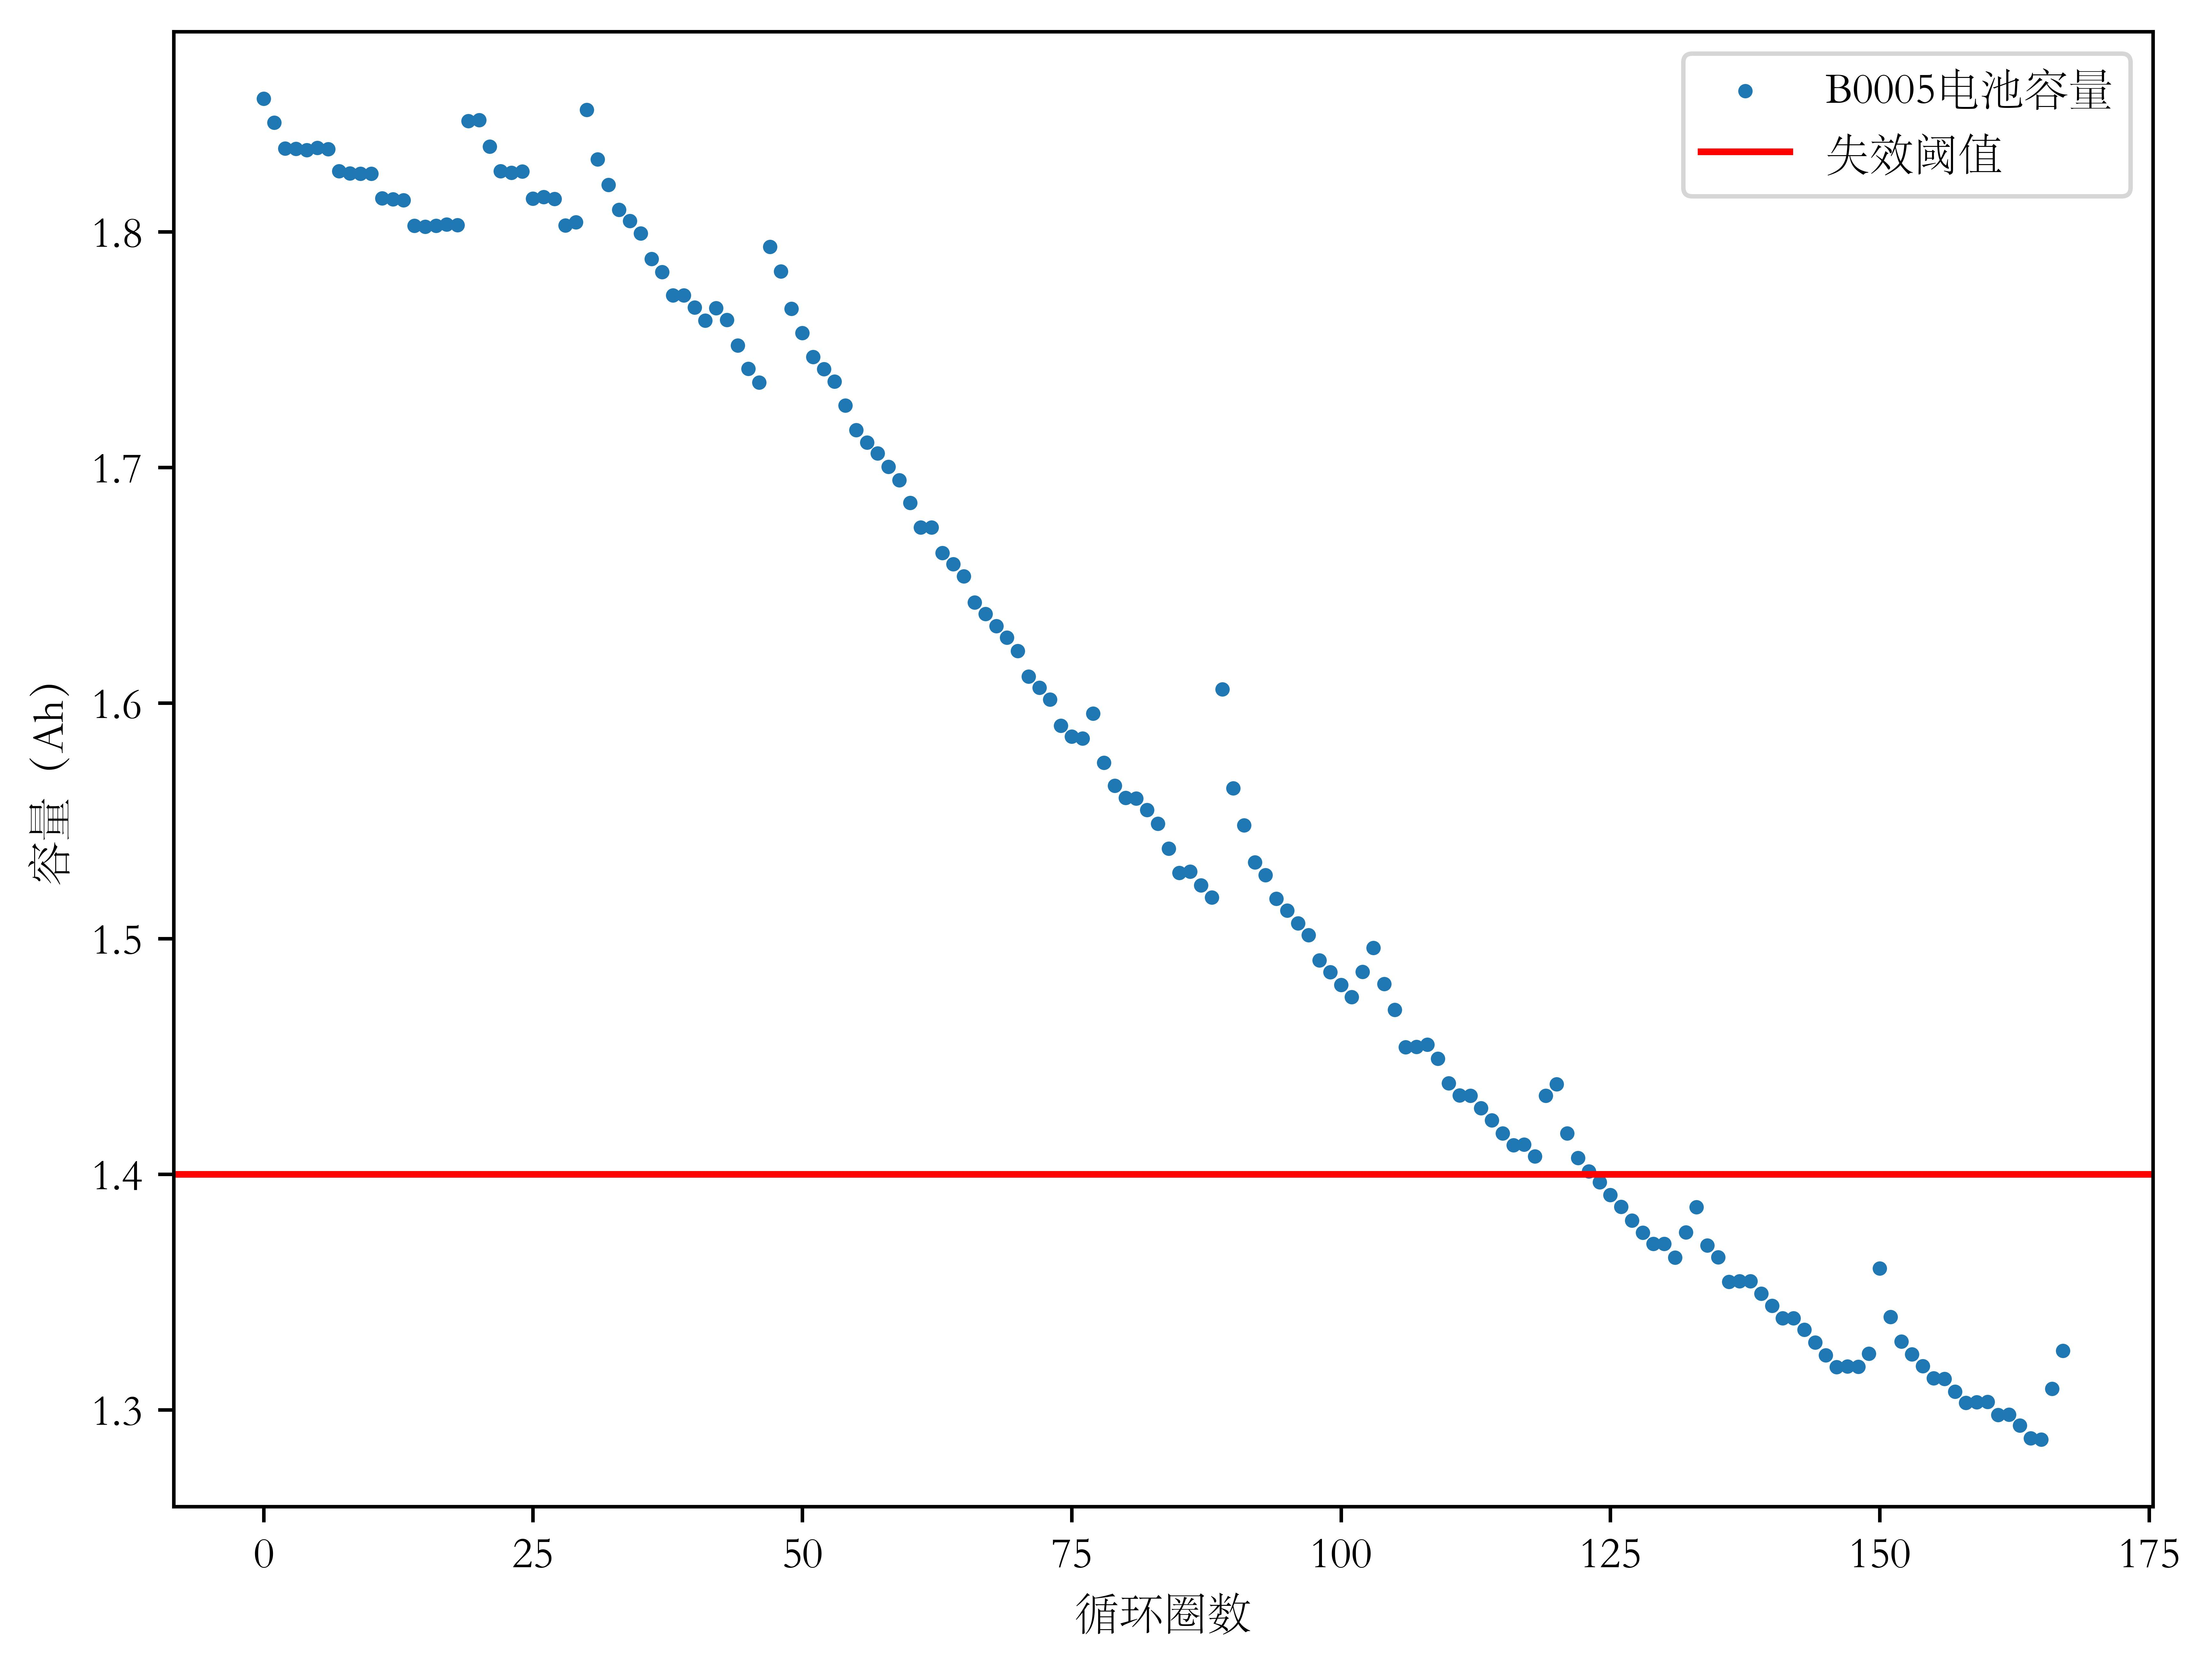
\includegraphics[scale=0.5]{figures/nasa_B0005_failure_threshold.jpg}
	\end{figure}
\end{frame}

\section{建模和实验}

\subsection{基于电池容量历史退化数据的SOH估计}

\subsection{基于电池充放电直接测量量的SOH估计}

\subsection{电池RUL预测}

\section{展望}

\begin{frame}
\begin{itemize}
\item 估计/预测模型改进
\item 模型在嵌入式平台的部署
\end{itemize}
\end{frame}

\section{写在最后}

\begin{frame}
	\centering
	本课题相关代码已在github上开源

	\centering
	\url {https://github.com/hilinxinhui/battery_phm.git}

	\begin{figure}[htbp]
		\centering
		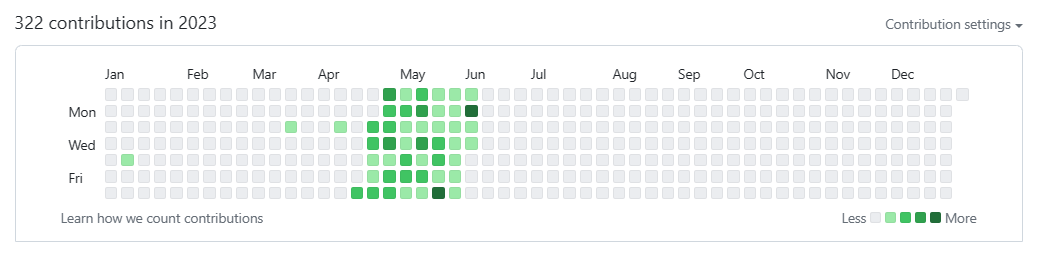
\includegraphics[scale=0.4]{figures/github_contribution_log.png}
		
	\end{figure}

\end{frame}

\begin{frame}
\begin{center}
{\Huge Thanks!}
\end{center}
\end{frame}

\end{document}
